\lecture{6}{10. September 2025}{Differential Analysis II: Kinematics \& Navier-Stokes equations}

\exercise{5.15}
A \qty{4}{m} diameter tank is filled with water and then rotated at a rate of $\omega = 2\pi \left( 1 - e^{-t} \right) \unit{s^{-1}}$. At the tank walls, viscosity prevents relative motion between the fluid and the wall. Determine the speed and acceleration of the fluid particles next to the tank walls as a function of time.
\bigbreak
We assume steady and incompressible flow. Due to viscosity the boundary condition at the tank wall requires that the velocity of the fluid particles right next to the walls must therefore be the same as that of the wall, i.e.
\[ 
V = \omega r = \frac{1}{2} \omega d = \frac{1}{2} \cdot 2\pi \left( 1 - e^{-t} \right) \unit{s^{-1}} \cdot \qty{4}{m} = 4\pi \left( 1 - e^{-t} \right) \unit{\frac{m}{s}}
.\]
The tangential acceleration is thus:
\[ 
  a_t = \frac{\mathrm{d}V}{\mathrm{d}t}  = 4 \pi e^{-t} \unit{\frac{m}{s^2}}
.\]
And the normal acceleration is:
\[ 
a_n = - \frac{V^2}{r} = - \frac{16 \pi^2 \left( 1 - e^{-t} \right)^2 \unit{\frac{m^2}{s^2}}}{\qty{2}{m}} = - 8 \pi^2 \left( 1 - e^{-t} \right)^2 \unit{\frac{m}{s^2}}
.\]



\exercise{5.19}
A velocity field is given $\textbf{V} = 2 \hat{i} - 4x \hat{j} \unit{\frac{m}{s}}$. Determine an equation for the streamline. Calculate the vorticity of the flow.
\bigbreak
The given velocity field is:
\begin{align*}
  u &= \qty{2}{\frac{m}{s}}  \\
  v &= - 4 x \unit{\frac{m}{s}}
.\end{align*}
To fund an equation for the streamline we use that the $x$ component of the velocity in terms of the stream function is:
\[ 
u = \frac{\partial \psi}{\partial y} = 2
.\]
By integrating with respect to $y$ we get
\[ 
\psi = 2y + f(x)
.\]
Doing the same for the $y$ component we get
\begin{align*}
  v &= -\frac{\partial \psi}{\partial x} = 4x \\
  \frac{\partial \psi}{\partial x} &= -4x \\
  \psi &= - 2x^2 + f(y)
.\end{align*}
Hence:
\[ 
\psi = 2y - 2x^2 + c
\]
where $c = \mathrm{constant}$. 

The vorticity of the flow is calculated as:
\[ 
  \boldsymbol{\xi} = \nabla \times \textbf{V} = \left( \frac{\partial v}{\partial x} - \frac{\partial u}{\partial y}  \right) \hat{k} = -4 \hat{k}
.\]


\exercise{5.22}
Consider a steady, laminar, fully developed incompressible flow between two infinite parallel plates as shown. The flow is due to a pressure gradient applied in the $x$-direction. Given that $\textbf{V} \neq \textbf{V}(z), w = 0$ and that gravity points in the negative $y$ direction, prove that $v = 0$ and that the pressure gradients in the $x$- and $y$-directions are constant.

\begin{figure} [ht]
  \centering
  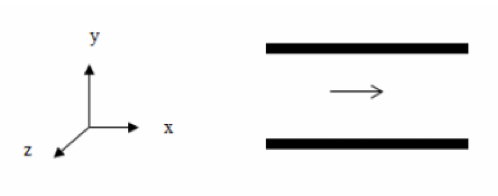
\includegraphics[width=0.5\linewidth]{./figures/f5_22.png}
\end{figure}
\bigbreak
For an incompressible steady flow the continuity equation simplifies to:
\[ 
\frac{\partial u}{\partial x} + \frac{\partial v}{\partial y} + \frac{\partial w}{\partial z}  = 0
.\]
And the momentum equations for the $x-$, $y-$, and $z$-directions are
\begin{align*}
  \rho \left( u \frac{\partial u}{\partial x} + v \frac{\partial u}{\partial y} + w \frac{\partial u}{\partial z}  \right)&= -\frac{\partial p}{\partial x} + \mu \left( \frac{\partial ^2 u}{\partial x^2} + \frac{\partial ^2 u}{\partial y^2} + \frac{\partial ^2 u}{\partial z^2}  \right) \\
    \rho \left( u \frac{\partial v}{\partial x} + v \frac{\partial v}{\partial y} + w \frac{\partial v}{\partial z}  \right)&= - \rho g -\frac{\partial p}{\partial y} + \mu \left( \frac{\partial ^2 v}{\partial x^2} + \frac{\partial ^2 v}{\partial y^2} + \frac{\partial ^2 v}{\partial z^2}  \right) \\
  \rho \left( u \frac{\partial w}{\partial x} + v \frac{\partial w}{\partial y} + w \frac{\partial w}{\partial z}  \right)&= -\frac{\partial p}{\partial z} + \mu \left( \frac{\partial ^2 w}{\partial x^2} + \frac{\partial ^2 w}{\partial y^2} + \frac{\partial ^2 w}{\partial z^2}  \right)
.\end{align*}
We have been informed that $w = 0$, $\textbf{V} \neq  \textbf{V}(z)$ and since the flow is fully developed we also have $\frac{\partial u}{\partial x} = 0$. Plugging this into the continuity equation we get:
\begin{align*}
  0 + \frac{\partial v}{\partial y} + 0 &= 0 \\
  \implies \frac{\partial v}{\partial y} &= 0
.\end{align*}
Therefore $v = \mathrm{constant}$. As $v = 0$ at the plate (for the continuity equation not to break for viscous flow) $v = 0$ everywhere.

From the momentum equation in the $z$-direction (since $w = 0$) we get:
\[ 
\frac{\partial p}{\partial z}  = 0
.\]
From the $y$-direction equation we get
\[ 
.\]
\begin{align*}
  \rho \left( u \cdot 0 + 0 \cdot 0 + 0\cdot 0 \right) &= - \rho g - \frac{\partial p}{\partial y}  \\
  0 &= - \rho g - \frac{\partial p}{\partial y}  \\
  \frac{\partial p}{\partial y} &= - \rho g \\
  \frac{\partial p}{\partial y} &= \mathrm{constant}
.\end{align*}
For the momentum equation in the $x$-direction we get
\begin{align*}
  \rho \left( u \cdot 0 + 0 \cdot \frac{\partial u}{\partial y} + 0 \cdot 0 \right) &= - \frac{\partial p}{\partial x} + \mu \left( 0 + \frac{\partial ^2 u}{\partial y^2} + 0 \right) \\
  0 &= - \frac{\partial p}{\partial x} + \mu \left( \frac{\partial ^2 u}{\partial y^2}  \right) \\
  \frac{\partial p}{\partial x} &= \mu \left( \frac{\partial ^2 u}{\partial y^2}  \right)
.\end{align*}
This is clearly not a function of $x$ and $z$ however it still could be a function of $y$. However as
\[ 
\frac{\partial p}{\partial y} = \mathrm{constant}
.\]
we know that $\frac{\partial p}{\partial x} $ cannot be a function of $y$. Hence $\frac{\partial p}{\partial x} = \mathrm{constant}$
